\chapter{\textbf{Конструкторский раздел}}

Задача этого проекта -- удостовериться, что пользователь отправляет валидный документ и дать ответ, какой тип документа он загрузил. 

Данное программное обеспечение предоставляет возможность классификации документов следующих типов. 
\begin{enumerate}
\item[1.] Паспорт гражданина Российской Федерации.
\begin{enumerate}
\item Первая страница -- когда и кем выдан.
\item Вторая страница -- фотография и личные данные.
\item Третья страница -- прописка.
\end{enumerate}
\item[2.] Водительское удостоверение.
\begin{enumerate}
\item Образец №1 -- ламинированное бумажное с 1995 по 2011.
\item Образец №2 -- пластиковое с 1995 по 2011.
\item Образец №3 -- удостоверение нового образца.
\end{enumerate}
\item[3.] Загранпаспорт гражданина Российской Федерации.
\item[4.] Шенгенская виза.
\begin{enumerate}
\item Франция.
\item Германия.
\item Италия.
\item Испания.
\end{enumerate}
\end{enumerate}

Классификатор получает входные данные: фотографию документа. На выходе классификатор сообщает, что он получил (паспорт, водительское удостоверение и так далее) и насколько он уверен в правильности ответа.

\newpage

\section{Функциональная модель}

На рисунке \ref{img:idef0} изображена функциональная модель, отображающая структуру и функции программного обеспечения. 

\begin{figure}[H]
	\centering
	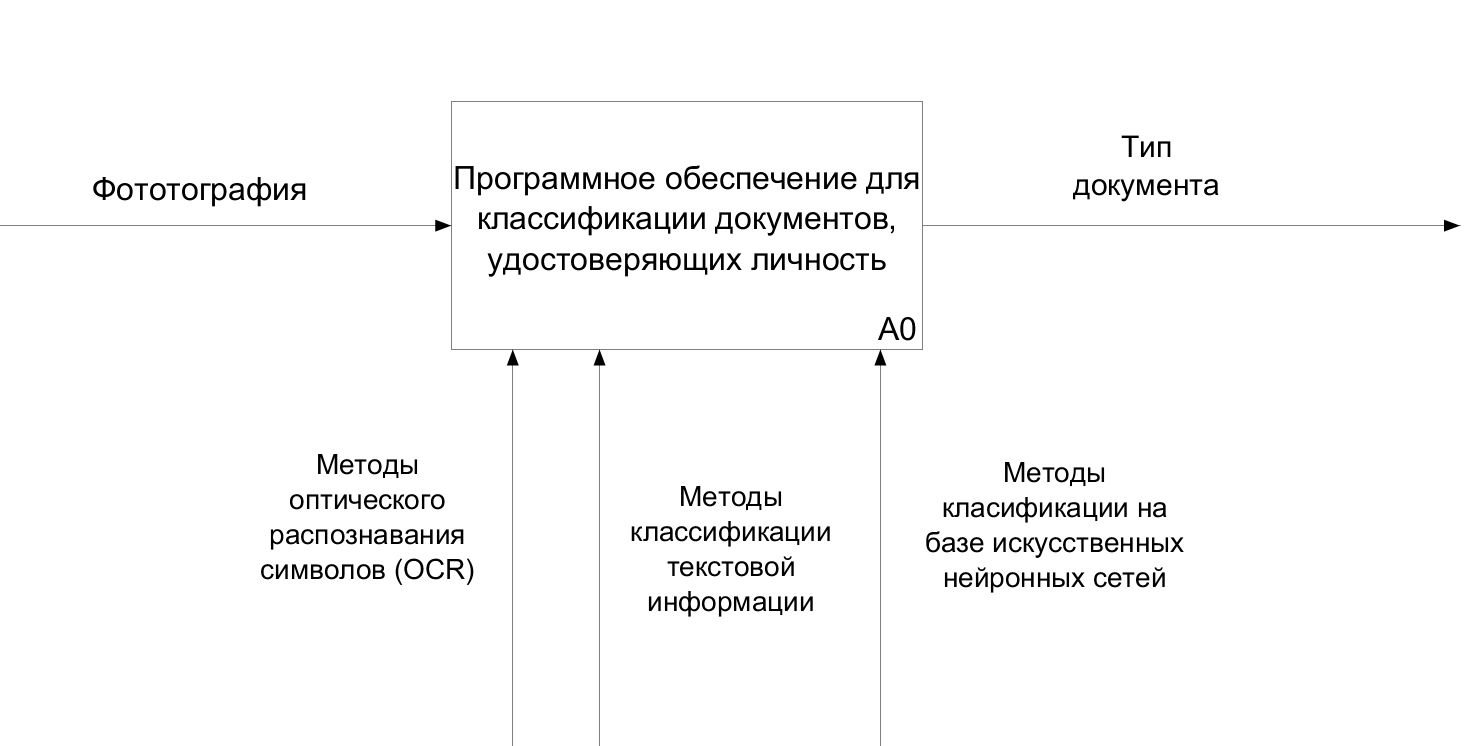
\includegraphics[scale=1.5]{idef0}
	\caption{Функциональная модель разрабатываемого ПО. }
	\label{img:idef0}
\end{figure}

На рисунке \ref{img:idef01} изображена функциональная модель первого уровня. 

\begin{figure}[H]
	\centering
	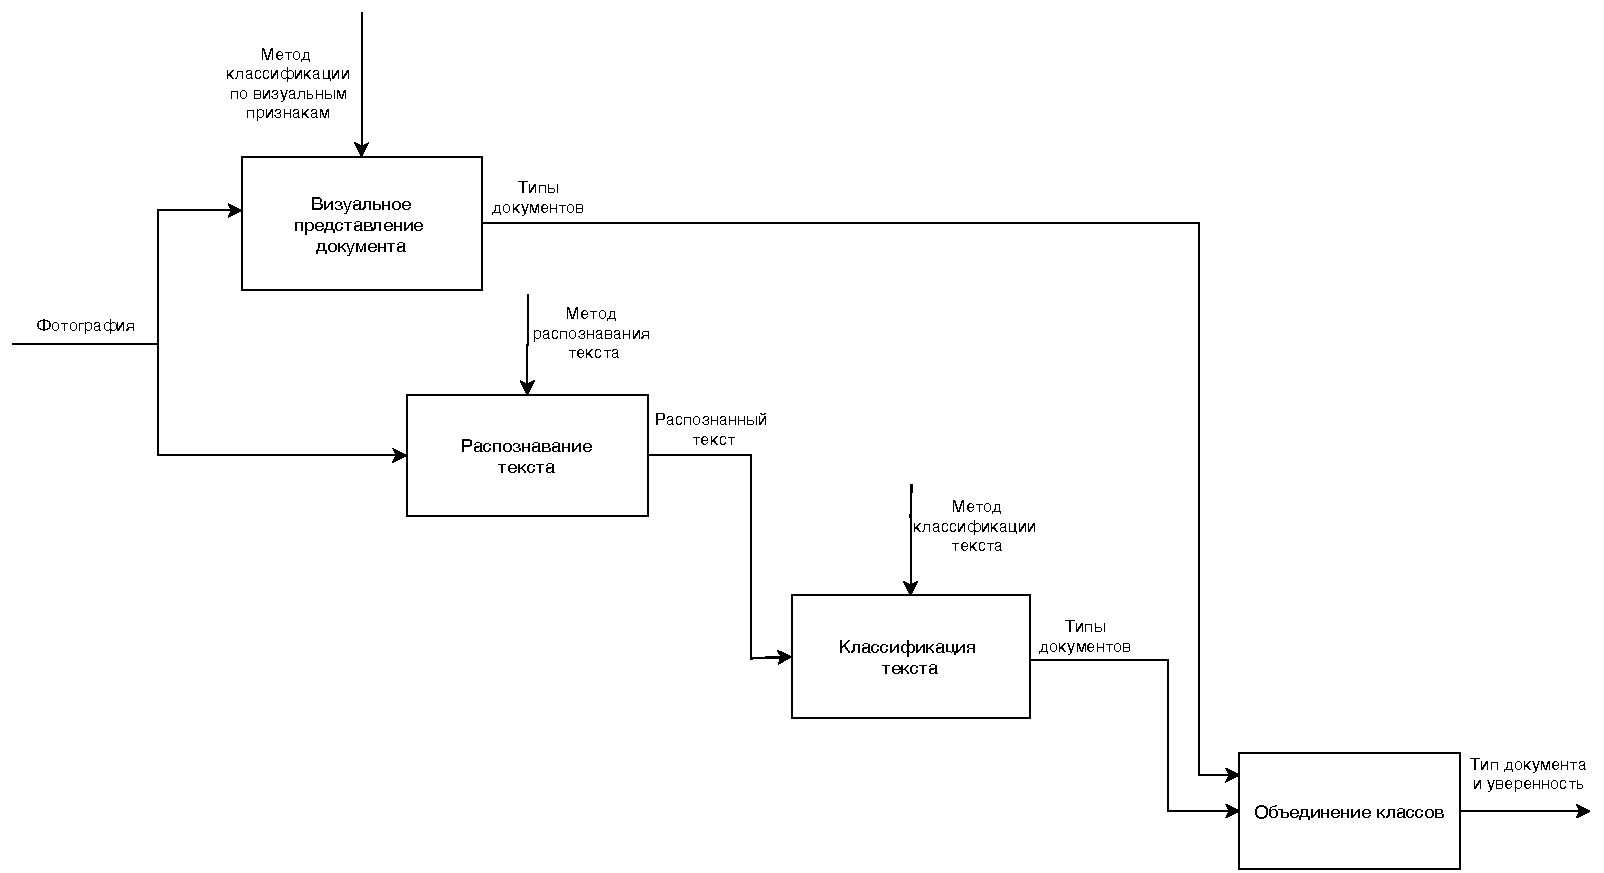
\includegraphics[scale=0.65]{idef01}
	\caption{Функциональная модель первого уровня. }
	\label{img:idef01}
\end{figure}
